\documentclass[main.tex]{subfiles}

\newcommand{\Par}{\operatorname{Parent}}
\newcommand{\LA}{\operatorname{LA}}
\newcommand{\Dep}{\operatorname{D}}
\newcommand{\LCA}{\operatorname{LCA}}

\newcommand{\NZ}{\operatorname{NZ}}
\newcommand{\CSB}{\textit{CSB}}
\renewcommand{\V}{\operatorname{V}}
\newcommand{\R}{\operatorname{R}}
\newcommand{\J}{\operatorname{J}}

\begin{document}

\chapter{LA com representação skew binary} \label{cap:skew}

Neste capítulo, apresentamos uma outra solução para o problema do Ancestral de Nível. Esta solução, apesar de um pouco mais complicada, requer processamento que consome espaço e tempo constante por nó adicionado. Está solução foi dada inicialmente por Myers~\cite{Myers83}.

\section{Definição e propriedades}

Um número \deff{skew-binary} de tamanho~$n$ é uma string~${a = a_n a_{n-1} \ldots a_1}$ tal que~${a_i \in \{0, 1, 2\}}$ e~$a_n \neq 0$. O valor de tal número é~${\V(a) \coloneqq \sum\limits_{i = 1}^n{a_i (2^i - 1)}}$. Note que múltiplas strings podem ter o mesmo valor, por exemplo, ambos~21 e~100 têm valor~7.

Para todo~$a$ tal que~$\V(a) \neq 0$, defina~$\NZ(a) \coloneqq \min\{i \in [n] : a_i \neq 0\}$, ou seja, a posição do dígito não nulo menos significativo de~$a$. Dizemos que um número skew-binary é \deff{canônico} se todos os seus dígitos são~0 ou~1 exceto, possivelmente, o dígito não nulo menos significativo. Mais formalmente, se~${a_i = 2 \implies i = \NZ(a)}$. Seja~$\CSB$ o conjunto de todos os números skew-binary.

Esta igualdade será útil na prova dos lemas:

\begin{equation} \tag{A} \label{eq:sum2}
	\sum\limits_{i = l}^r{2^i} = 2^{r+1} - 2^{l}.
\end{equation}

\begin{lemma} \label{lem:csbdig}
	Se~$a \in \CSB$ e~$|a| = n$, então~$2^n - 1 \leq \V(a) \leq 2^{n+1}-2$.
\end{lemma}
\begin{proof}
	Considere o número~$b = 10^{n-1}$. Como, por definição,~$a_n \geq 1 = b_n$ e~$a_i \geq 0 = b_i$ para~$i \in [n - 1]$, vale que~$V(b) \geq V(a) = 2^n - 1$.

	Note que
	\begin{align*}
	V(a) = \sum\limits_{i = \NZ(a)}^n{a_i (2^i - 1)} &\stackrel{\text{(1)}}{\leq} \left(\sum\limits_{i = \NZ(a) + 1}^n (2^i - 1)\right) + 2 (2^{\NZ(a)} - 1) \\
	&\stackrel{\text{(2)}}{=} 2^{n+1} - 2^{\NZ(a)+1} - (n - \NZ(a)) + 2^{\NZ(a) + 1} - 2 \\
	&\stackrel{\text{(3)}}{\leq} 2^{n+1} - 2,
	\end{align*}
	onde~(1) vale por que~$a \in \CSB$,~(2) vale por~\eqref{eq:sum2} e~(3) vale pois~$\NZ(a) \leq n$.

\end{proof}

O lema mostra que o menor e maior número de~$n$ dígitos em CSB são~$10^{n-1}$ e~$20^{n-1}$, respectivamente, e também que qualquer representação de~$x$ em CSB usa~$\floor{\lg(x + 1)}$ dígitos.

\begin{theorem} \label{thm:csbbij}
	Cada número tem uma representação única em CSB. Equivalentemente,~${\V: \CSB \rightarrow \mathbb{N}}$ é uma função bijetora.
\end{theorem}
\begin{proof}
	Vamos provar que~$\V$ é injetora, ou seja, se~${a \neq b}$ então~${\V(a) \neq \V(b)}$. Suponha, sem perda de generalidade, que~$|a| \geq |b|$. Se~$|a| > |b|$, então, pelo~Lema~\ref{lem:csbdig},
	$$ \V(a) \geq 2^{|a|} - 1 > 2^{|a|} - 2 \geq 2^{|b| + 1} - 2 \geq \V(b). $$
	Se~$|a| = |b|$, considere~${i^\star = \max\{i \in [n] : a_i \neq b_i\}}$. Assuma, sem perda de generalidade, que~${a_{i^\star} > b_{i^\star}}$. Escreva~${a = \alpha a_{i^\star} \beta}$ e~${b = \alpha b_{i^\star} \gamma}$. Então
	$$ V(a) - V(b) \stackrel{\text{(1)}}{\geq} (2^{i^\star} - 1) + V(\beta) - V(\gamma) \stackrel{\text{(2)}}{\geq} (2^{i^\star} - 1) - (2^{i^\star} - 2) = 1, $$
	onde~(1) vale pois~$a_i \geq b_i + 1$,~(2) vale pois~$\V(\beta) \geq 0$ e usando o Lema~\ref{lem:csbdig} sobre~$\gamma$. Isso prova que~$\V(a) \neq \V(b)$, logo~$\V$ é injetora.

	Para provar que~$\V$ é sobrejetora, precisamos provar que, para todo~$x \in \mathbb{N}$, existe~$a \in \CSB$ tal que~$V(a) = x$. Por indução em~$n$, vamos provar que, para todo~$x \leq 2^{n+1} - 2$ existe~$a \in \CSB$ tal que~$V(a) = x$. Se~$n = 0$, então~$a = 0$ é tal que~$V(a) = 0$. Suponha que a hipótese vale para todo~$x \leq 2^n - 2$. Seja~${2^n - 1 \leq y \leq 2^{n+1} - 2}$. Se~$y = 2^{n+1} - 2$, sabemos que~${a = 20^{n-1} \in \CSB}$ é tal que~$V(a) = y$. Caso contrário,~
	$$y - (2^n - 1) < 2^{n+1} - 2 - (2^n - 1) = 2^n - 1,$$
	logo existe~$a \in \CSB$ tal que~${V(a) = y - (2^n - 1)}$, mas então~$b = 1a \in \CSB$ e~$V(b) = y$.
\end{proof}

Como cada número tem uma representação única em~CSB, podemos definir uma função~${\R: \mathbb{N} \rightarrow \CSB}$ tal que~$V(\R(x)) = x$ para todo~$x \in \mathbb{N}$.

\begin{lemma} \label{lem:csbsub}
	Seja~$a \in \CSB$ tal que~$\V(a) > 0$. Se~$\NZ(a) = 1$ então~$V(a_n \ldots a_2 (a_1-1)) = V(a) - 1$, caso contrário~${V(a_n \ldots a_{\NZ(a)+1} (a_{\NZ(a)} - 1) 2 0^{\NZ(a) - 2}) = V(a) - 1}$.
\end{lemma}
\begin{proof}
	Quando~$\NZ(a) = 1$, vale que~$a_1 \neq 0$, logo~${b \coloneqq a_n \ldots a_2 (a_1-1) \in \CSB}$. Além disso,~${V(a) - V(b) = a_1 - b_1 = 1}$.

	Caso contrário,~${a_{\NZ(a)} \neq 0}$, e como o único dígito em~$a$ que pode ser~2 é o~$\NZ(a)$-ésimo dígito, temos que~${b \coloneqq a_n \ldots a_{\NZ(a)+1} (a_{\NZ(a)} - 1) 2 0^{\NZ(a) - 2} \in \CSB}$. Além disso,
	$$ V(a) - V(b) = (a_{\NZ(a)} - b_{\NZ(a)}) (2^{\NZ(a)} - 1) - 2 (2^{\NZ(a) - 1} - 1) = 2^{\NZ(a)} - 1 - (2^{\NZ(a)} - 2) = 1. $$
\end{proof}

O lema mostra que subtração por~1 em skew-binary canônico consiste de diminuir em 1 o dígito não nulo menos significativo e, se existir, aumentar para~2 o dígito à direita deste.

\section{Jump pointers}

No problema do Ancestral de Nível, para avaliar~$\LA(k, u)$, temos um nó~$u$ de profundidade~$\Dep(u)$ e queremos determinar seu ancestral~$v$ de profundidade~${\Dep(v) = \Dep(u) - k}$. Na solução apresentada na Subseção~\ref{subsec:pot2}, cada nó tinha um ponteiro para seu $2^x$-ancestral, para todo~${x \in \floor{\lg\Dep(u)}}$, e o nó~$v$ era alcançado a partir de~$u$ pulando as potências de dois distintas da decomposição de~$k$.

Este problema pode ser interpretado de outra forma. Temos um número~$x$ e queremos transformá-lo em~$y \leq x$, a cada passo diminuindo o valor de~$x$. Com esta interpretação, na solução da Subseção~\ref{subsec:pot2}, que tenta transformar~$\Dep(u)$ em~$\Dep(v)$, a partir de cada número podíamos subtrair qualquer potência de dois. Note que diminuir o valor de um número por~$z$ é equivalente a escolher o~$z$-ésimo ancestral de um nó.

Vamos considerar uma solução alternativa para este problema, na qual partir de um número~$x$ positivo podemos pular para os números~$x-1$ ou~$\J(x)$, onde~${\J(x) \coloneqq x - (2^{\NZ(\R(x))} - 1)}$, ou seja, se considerarmos~$\R(x)$, a representação em~skew-binary canônico de~$x$,~$\J(x)$ consiste de diminuir em um o dígito não nulo menos significativo de~$\R(x)$. Por exemplo, se~$x = 13$, então~${\R(x) = 120}$ e~${\J(x) = \V(110) = 10}$.

Considere o seguinte algoritmo, que transforma~$x$ em~$y$ (inicialmente~$x > y$):
\begin{algorithm}[h]
\caption{Transformando~$x$ em~$y$ usando~$x-1$ e~$\J(x)$. \label{lst:xysub}}
\begin{algorithmic}[1]
	\While{$x \neq y$}
		\If{$\J(x) \geq y$}
			\State $x = \J(x)$
		\Else
			\State $x = x - 1$
		\EndIf
	\EndWhile
\end{algorithmic}
\end{algorithm}

O algoritmo é guloso no sentido que sempre escolhe usar~$\J$ quando possível (e~${\J(x) \leq x - 1}$). A correção do algoritmo é clara, já que é sempre possível alcançar~$y$ usando apenas~$x-1$, e~$x$ nunca se torna menor que~$y$.

\begin{theorem} \label{thm:xysub}
	O algoritmo no Código~\ref{lst:xysub} termina em~$\Oh(\lg x)$ iterações do~\keyword{while}.
\end{theorem}
\begin{proof}
	Seja~$a \coloneqq \R(x)$ e~$b \coloneqq \R(y)$ e~$n \coloneqq |a|$. Se~$|a| > |b|$, aumente~$b$ adicionando 0s à esquerda. Seja~${i^\star = \max\{i \in [n] : a_i \neq b_i\}}$, e escreva~${a = \alpha a_{i^\star} \beta}$ e~${b = \alpha b_{i^\star} \gamma}$. Pelo Lema~\ref{lem:csbdig} (e também usado na prova do Teorema~\ref{thm:csbbij}), temos que~$a_{i^\star} > b_{i^\star}$ e que~${V(c) > V(b)}$, onde~${c \coloneqq b_n \ldots b_{i^\star + 1} (b_{i^\star} + 1) 0^{i^\star - 1}}$. Note que~$c_i \leq a_i$ para todo~${i \in [n]}$, e temos que~$\NZ(a) \leq i^\star$. Se~$\NZ(a) < i^\star$ vale que~$a_{\NZ(a)} > 0 = c_{\NZ(a)}$, e se~$\NZ(a) = i^\star$ vale que~${a_{\NZ(a)} = a_{i^\star} \geq b_{i^\star} + 1 = c_{i^\star}}$. Portanto~$a_{\NZ(a)} \geq c_{\NZ(a)}$, com igualdade apenas se~$a = c$, logo se~$a \neq c$ podemos diminuir~$a_{\NZ(a)}$ em um, ou seja,~$J(V(a)) \geq V(c)$. Podemos repetir este argumento até que~$a = c$, ou seja~$x = V(c)$. Esta parte realiza no máximo~${\sum\limits_{i = 1}^{i^\star}{a_i} \leq i^\star + 1}$ iterações, já que cada dígito é no máximo~1, a menos de um destes, que pode ser~2.

	Vamos provar que, se~${a = b_n \ldots b_{i+1} (b_i + 1) 0^{i-1}}$ para algum~$1 \leq i \leq n$, com~$x = \V(a)$ e~$y = \V(b)$, então o algoritmo terminará em no máximo~$2i$ iterações. Com isso provado, começando de~${c = b_n \ldots b_{i^\star + 1} (b_{i^\star} + 1) 0^{i^\star - 1}}$, o algoritmo realiza no máximo~$2i^\star$ iterações adicionais, logo o algoritmo realiza no máximo~${3i^\star + 1 \leq 3n+1 = \Oh(\lg x)}$ iterações no total, e o teorema estará provado.

	A prova será por indução em~$i$. Se~$i = 1$ então~${J(x) = x - 1 = y}$ e o algoritmo termina em uma iteração.

	Suponha que a hipótese vale para valores menores que~$i$. Se~${\NZ(b) \geq i}$, ou seja,~$b$ tem um sufixo de pelo menos~$i - 1$ valores 0, ou seja~${a = b_n \ldots b_{i + 1} (b_{i} + 1) b_{i - 1} \ldots b_1}$, e então se diminuirmos~1 de~$a_{i}$ temos~$b$, ou seja,~${\J(\V(a)) = \V(b)}$, e o algoritmo termina em uma iteração.
	Caso contrário,~$\J(\V(a)) < \V(b)$, e então~$x = x - 1$ é executado. Pelo Lema~\ref{lem:csbsub},~${\R(x - 1) = b_n \ldots b_i 2 0^{i-2}}$, e é claro que~${\V(20^{i-2}) \geq \V(b_{i-1} \ldots b_1)}$. Considere o valor de~$b_{i-1}$:
	\begin{itemize}
		\item se~$b_{i-1} = 2$, então~$x - 1 = y$ e o algoritmo termina, gastando uma iteração;
		\item se~$b_{i-1} = 1$, então podemos aplicar a hipótese de indução (para~$i-1$) e temos que o algoritmo gasta no máximo~$2(i - 1) + 1 < 2i$ iterações;
		\item se~$b_{i-1} = 0$, então~$\J(x - 1) > y$ e~$\R(\J(x - 1)) = b_n \ldots b_i 1 0^{i-2}$, logo podemos aplicar a hipótese de indução (para~$i-1$) e temos que o algoritmo gasta no máximo~$2(i-1) + 2 = 2i$ iterações.
	\end{itemize}
\end{proof}

\begin{figure}
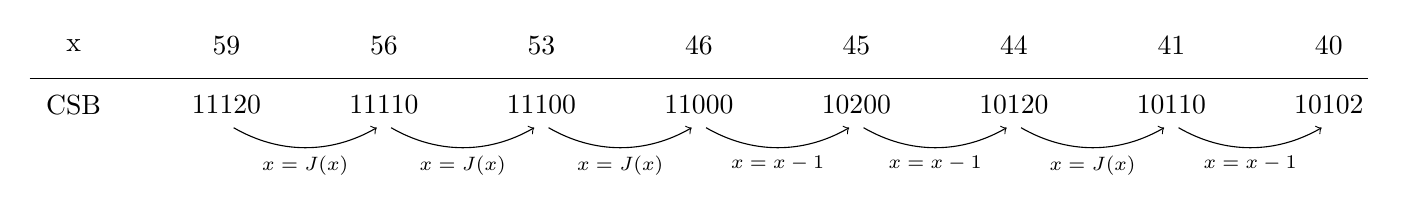
\begin{tikzpicture}
	%\draw (0, 1/10) node{x\ \ \ \ CSB\ \ };
	\draw (0, 3/4) node{\ \ x\ \ };
	\draw (0, 0) node{\ CSB\ };
	%\draw (0, 0) grid (20, 10);
	\draw (-.5, 1/3) -- (16.5, 1/3);
	\foreach \i/\x/\csb in {1/59/11120, 2/56/11110, 3/53/11100, 4/46/11000, 5/45/10200, 6/44/10120, 7/41/10110, 8/40/10102}
	{
		\draw (\i+\i, 3/4) node{\ \x\ \ };
		\draw (\i+\i, 0) node(c\i){\csb};
	}
	\foreach \i/\j in {1/2, 2/3, 3/4, 6/7}
	{
		\draw (c\i.south) edge[bend right,->, shorten >=3pt, shorten <=3pt] node[below]{\scriptsize $x = \J(x)$} (c\j.south);
	}
	\foreach \i/\j in {4/5, 5/6, 7/8}
	{
		\draw (c\i.south) edge[bend right,->, shorten >=3pt, shorten <=3pt] node[below]{\scriptsize $x = x - 1$} (c\j.south);
	}
\end{tikzpicture}
\caption{Exemplo do algoritmo do Código~\ref{lst:xysub} aplicado sobre~$x = 59$ e~$y = 40$.} \label{fig:exxysub}
\end{figure}

A Figura~\ref{fig:exxysub} mostra um exemplo de aplicação do algoritmo no Código~\ref{lst:xysub}. A transformação de~$x = 59$ até~$x = 46$ corresponde à primeira parte da prova do Teorema~\ref{thm:xysub}, e o resto corresponde à segunda.

\newcommand{\jmp}{\mathit{jump}}
Portanto, é possível usar a mesma ideia para resolver o problema do Ancestral de Nível. Suponha que todo vértice~$u$ tenha um campo~$u.\jmp$ que armazene seu ancestral com profundidade~$\J(\Dep(u))$. Então, de forma análoga ao algoritmo do Código~\ref{lst:xysub}, podemos resolver o problema do Ancestral de Nível como no Código~\ref{lst:laskew}. A correção é clara e o consumo de tempo~$\Oh(\lg\Dep(u))$ segue diretamente do Teorema~\ref{thm:xysub}.

\begin{algorithm}
\caption{Algoritmo para Ancestral de Nível usando a representação skew-binary.} \label{lst:laskew}
\begin{algorithmic}[1]
	\Function{LevelAncestor}{$k, u$}
		\State $y = \Dep(u) - k$
		\While{$\Dep(u) \neq y$}
			\If{$\Dep(u.\jmp) \geq y$}
				\State $u = u.\jmp$
			\Else
				\State $u = \Par(u)$
			\EndIf
		\EndWhile
		\State \Return $u$
	\EndFunction
\end{algorithmic}
\end{algorithm}

\section{Computando jump pointers}

A seção anterior apresentou uma solução para o problema do Ancestral de Nível que consome tempo logarítmico, porém, assumimos que cada nó~$u$ tinha um campo~$u.\jmp$ com seu~$\J(\Dep(u))$-ésimo ancestral. Nesta seção, detalharemos como encontrar tal ancestral para cada nó.

\begin{theorem} \label{thm:csbj+1}
	Seja~$a \in \CSB$. Se~$a$ não contém nenhum dígito dois, ou seja, se~$a_{\NZ(a)} \neq 2$, então~$\J(\V(a) + 1) = \V(a)$. Caso contrário,~$\J(\V(a) + 1) = \J(\J(\V(a))$.
\end{theorem}
\begin{proof}
	Suponha que~$a_{\NZ(a)} \neq 2$. Note que~$b \coloneqq a_n \ldots a_2 (a_1 + 1)$ é um número em skew-binary tal que~${\V(b) = \V(a) + 1}$, e, já que~$a$ não tem dígito~2, vale que~${b \in \CSB}$. Obviamente~${\NZ(b) = 1}$, logo~${\J(\V(a) + 1) = \J(\V(b)) = \V(b) - 1 = \V(a)}$.

	Caso contrário,~${a_{\NZ(a)} = 2}$. Considere~${b \coloneqq a_n \ldots a_{\NZ(a) + 2} (a_{\NZ(a) + 1} + 1) 0^{\NZ(a)}}$, pelo Lema~\ref{lem:csbsub} vale que~${R(V(b) - 1) = a}$, logo~${V(b) = V(a) + 1}$. Note que \vspace{-2ex}
	\[
	\begin{array}{ll}
		\J(\V(b))     &= a_n \ldots a_{\NZ(a) + 1} 0^{\NZ(a)}, \\
		\J(\V(a))     &= a_n \ldots a_{\NZ(a) + 1} 10^{\NZ(a)-1},\text{ e} \\
		\J(\J(\V(a))) &= a_n \ldots a_{\NZ(a) + 1} 0^{\NZ(a)}. \\
	\end{array}
	\]
	Portanto,~$\J(V(a) + 1) = \J(\J(\V(a)))$.
\end{proof}

Pelo Teorema~\ref{thm:csbj+1}, é fácil calcular~$\J(x)$ a partir dos valores~$\J$ calculados para valores menores que~$x$, se soubermos identificar se~$\R(x - 1)$ tem algum dígito~2.

\begin{proposition} \label{prop:csbjj}
	Seja~$a \in \CSB$ tal que~$\V(a) \neq 0$. Então \vspace{-2ex}
	$${a_{\NZ(a)} = 2 \iff \J(\V(a)) \neq 0 \text{ e } \V(a) - \J(\V(a)) = \J(\V(a)) - \J(\J(\V(a))).}$$
\end{proposition}
\begin{proof}
	Seja~$b \coloneqq \R(\J(\V(a)))$ e~${c \coloneqq \R(\J(\V(b)))}$. Lembre que~${\J(\V(a)) = \V(a) - (2^{\NZ(a)} - 1)}$.

	Se~$a_{\NZ(a)} = 2$, então~$\NZ(b) = \NZ(a)$ (e~$\V(b) \neq 0$), logo segue que~$$\V(a) - \J(\V(a)) = 2^{\NZ(a)} - 1 = 2^{\NZ(b)} - 1 = \V(b) - \J(\V(b)) = \J(\V(a)) - \J(\J(\V(a))).$$

	Já se~$a_{\NZ(a)} = 1$, então se~$\J(\V(a)) \neq 0$ vale que~$\NZ(b) > \NZ(a)$, logo segue que~$$\V(a) - \J(\V(a)) = 2^{\NZ(a)} - 1 < 2^{\NZ(b)} - 1 = \V(b) - \J(\V(b)) = \J(\V(a)) - \J(\J(\V(a))).$$
\end{proof}

A Proposição~\ref{prop:csbjj} nos dá uma maneira de verificar se a representação skew-binary de~$x$ tem algum dígito~2, se já tivermos calculado os valores de~$\J$ para números menores ou iguais a~$x$.

\renewcommand{\root}{\mathit{root}}
\begin{algorithm}
\caption{Adicionando uma folha à árvore com raiz~$r$.} \label{lst:addleafskew}
\begin{algorithmic}[1]
	\Function{\API{AddLeaf}}{$u$}
		\State $v = \Par(u)$
		\If{$v.\jmp \neq r \textbf{ and } \Dep(v) - \Dep(v.\jmp) = \Dep(v.\jmp) - \Dep(v.\jmp.\jmp)$} \label{lst:addleafskew:if}
			\State $u.\jmp = v.\jmp.\jmp$
		\Else
			\State $u.\jmp = v$
		\EndIf
	\EndFunction
\end{algorithmic}
\end{algorithm}

O Código~\ref{lst:addleafskew} mostra como adicionar uma folha de forma online à árvore, da mesma forma como no Código~\ref{lst:lapot2}. Nesse caso, porém, o consumo de tempo e espaço é constante. A correção segue diretamente do Teorema~\ref{thm:csbj+1} e da Proposição~\ref{prop:csbjj}, já que a comparação da linha~\nref{lst:addleafskew:if} verifica as condição dadas pela proposição e o~\keyword{if} computa o campo~$\jmp$ (equivalente à função~$\J$) como no teorema. Note que a raiz~$r$ tem profundidade~0 e seu campo~$\jmp$ não é usado.

\section{Ancestral comum mais profundo}

Para encontra o ancestral comum mais profundo de dois vértices~$u$ e~$v$, usamos a mesma lógica descrita na Seção~\ref{sec:lca_pot2}. Inicialmente nivelamos~$u$ e~$v$ para terem a mesma profundidade. Seja~$c$ o ancestral comum mais profundo de~$u$ e~$v$, note que no Código~\ref{lst:xysub} não é realmente necessário conhecermos~$y$, apenas precisamos determinar, a cada iteração, se~$\J(x) \geq y$. Sabemos que~${u.\jmp = v.\jmp \iff D(u.\jmp) > D(c)}$, ou seja, podemos determinar se~${J(D(u)) \geq D(c) + 1}$.

Dessa forma, conseguimos encontrar o ancestral de~$u$ com profundidade~$D(c) + 1$, e o pai deste será~$c$. Veja o Código~\ref{lst:lca_skew}, e note sua similaridade com o Código~\ref{lst:lcapot2}.

\begin{algorithm}
\caption{Ancestral Comum Mais Profundo usando representação skew-binary \label{lst:lca_skew}}
\begin{algorithmic}[1]
	\Function{\API{LowestCommonAncestor}}{$u, v$}
		\If{$\Dep(u) > \Dep(v)$}
			\State $u, v = v, u$ \Comment{Garantindo que~$\Dep(u) \leq \Dep(v)$.}
		\EndIf
		\State $v = \funcAPI{LevelAncestor}{\Dep(v) - \Dep(u), v}$ \Comment{Nivelando~$v$.}
		\If{$u = v$}
			\State \Return $u$
		\EndIf
		\While{$\Par(u) \neq \Par(v)$}
			\If{$u.\jmp \neq v.\jmp$}
				\State $u = u.\jmp$
				\State $v = v.\jmp$
			\Else
				\State $u = \Par(u)$
				\State $v = \Par(v)$
			\EndIf
		\EndWhile
		\LineComment{$u$ é agora o filho do LCA de~$u$ e~$v$.}
		\State \Return $\Par(u)$
	\EndFunction
\end{algorithmic}
\end{algorithm}

A Tabela~\ref{tab:la_skew} mostra o consumo de tempo e espaço das implementações discutidas nesse capítulo. A Tabela~\ref{tab:la_comp} compara o consumo de tempo das implementações de~Ancestral de Nível e Ancestral Comum Mais Profundo apresentadas nesse trabalho.

\begin{table} \centering
\begin{tabular}{|l|c|}
	\hline
	& Tempo/Espaço \\ \hline
	\funcAPI{AddLeaf}{u} & $\Oh(1) / \Oh(1)$ \\
	\funcAPI{LevelAncestor}{k, u} & $\Oh(\lg n) $ \\
	\funcAPI{LowestCommonAncestor}{u, v} & $\Oh(\lg n)$ \\ \hline
\end{tabular}
	\caption{Consumo de tempo e espaço da solução com skew-binary, onde~$n$ é o tamanho da árvore.} \label{tab:la_skew}
\end{table}

\begin{table}[H] \centering
\begin{tabular}{|l|c|c|}
	\hline
	& Representação binária & Skew-binary \\ \hline
	\funcAPI{AddLeaf}{u} & $\Oh(\lg n) / \Oh(\lg n)$ & $ \Oh(1) / \Oh(1)$ \\
	\funcAPI{LevelAncestor}{k, u} & $\Oh(\lg n) $ & $\Oh(\lg n) $ \\
	\funcAPI{LowestCommonAncestor}{u, v} & $\Oh(\lg n)$ & $\Oh(\lg n) $ \\ \hline
\end{tabular}
	\caption{Comparação do consumo de tempo e espaço das soluções dos Capítulos~\ref{cap:ancestrais} e~\ref{cap:skew}, onde~$n$ é o tamanho da árvore.} \label{tab:la_comp}
\end{table}


\end{document}
